\newpage
\section{DNA sequencing}
In DNA sequencing there are a lot of technologies involved.
In particular an output from the DNA sequencer is composed by:

\begin{itemize}
  \item Raw data (for instance the fluorescent images taken by the sequencer)
  \item Sequencing data
  \item Metadata (informations about the experiment itself)
\end{itemize}

The sequencing data are:
\begin{itemize}
	\item Reads (base space or color space)
	\item Quality file
\end{itemize}

These informations can be stored in two separate multi-fasta files or in a
single fastq file, as shown later.

The most common way to save data is in the \textit{fasta} format. The quality is
usually saved in a \textit{qual} format, with the same name of the
\textit{fasta} file. For each base there is a point, that measure the quality.
The quality is: $Q=-10\log_{10}P$

\paragraph*{How to calculate the P value} With machine learning you can
calculate the probability to have bad or good reads. \\

\begin{figure}[H]
  \centering
  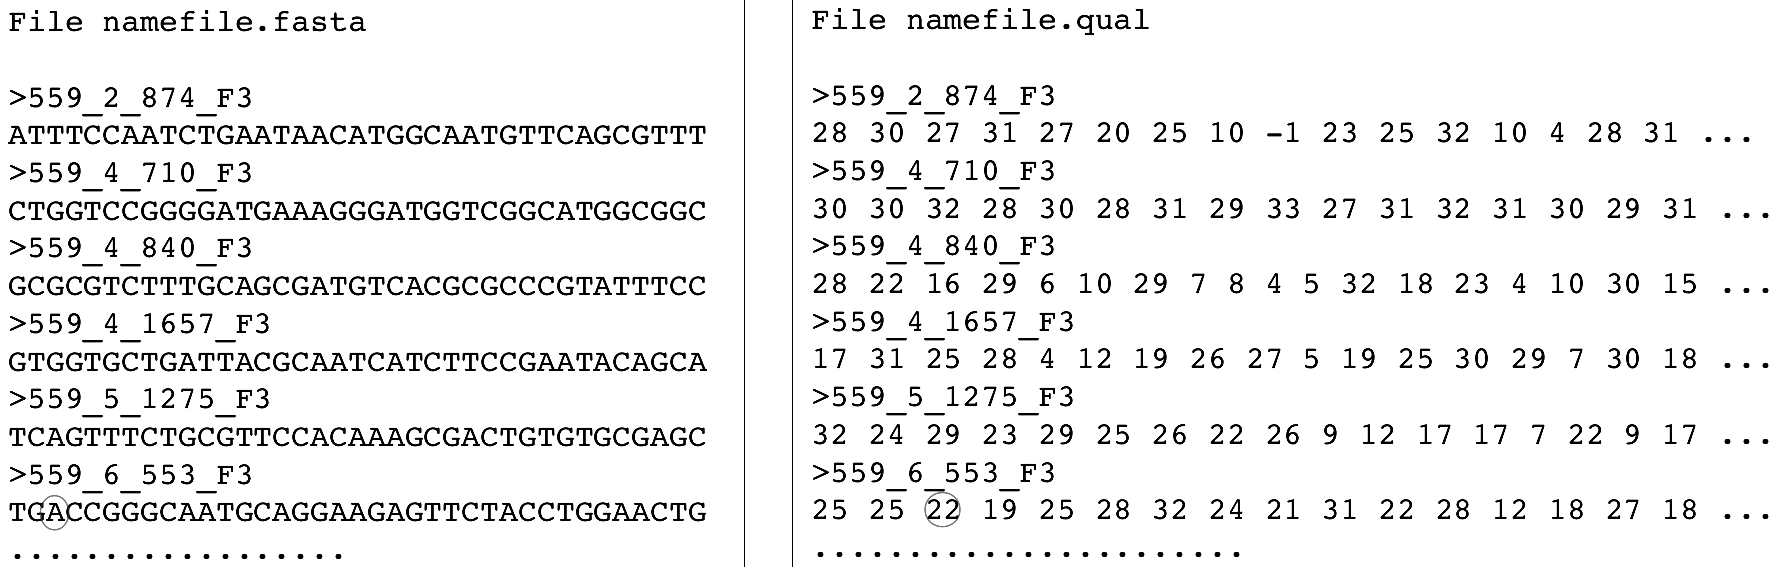
\includegraphics[scale=0.25]{fastaqual}
  \caption{FASTA and QUALITY files}
  \label{fig:fastaqual}
\end{figure}

It is difficult to correlate the reads with their quality values, no matter if checked by human or by machine.
Is there any way to make it easier?

During the years people found that \textit{fasta} and \textit{qual} format were
difficult to read. So a new format was inventend around 2000: \textit{FASTQ}.
The fastq format allows to store both sequence and quality in the same file.
The quality is stored using one symbol per value.
The new format is composed by:
\begin{itemize}
  \item Sequence id
  \item Genome sequence
  \item A line for comment (starting with +). It can be empty
  \item A line for quality. The quality is encoded with ASCII char, where the
first char (with quality equal to 0) starts from 33 (!) and finish with 126.
This line must obviously contain the same number of symbols as letters in
the sequence.
\end{itemize}

The reads can be from different sources

\begin{itemize}
	\item DNA is from genomic fragments
	\item DNA is from PCR amplicons
	\item DNA is from RNA retrotranscribed into cDNA
\end{itemize}

The jobs to be performed may be different

\begin{itemize}
	\item De novo genomic assembly
	\item Genomic resequencing
	\item Finding somatic or viral variants
	\item Quantify gene expression (RNA-seq)
	\item Single-base resolution RNA profiling
	\item De novo transcriptome assembly 
\end{itemize}

\section{Alignment of reads on a reference genome}

One of the most common task to be performed on NGS reads is the alignment on a reference genome.
The reads can have several origins: RNA, genome, ChIP, and more.
Depending on the type of project, it may be useful to use different alignment strategies;
for instance transcripts should align over splicing sites,
while genomic DNA should not.
Moreover, the reads could be single-reads, pairends or mate-pairs.
Let's consider the simplest task: the alignment of genomic fragments on a reference genome.

\begin{figure}[H]
  \centering
  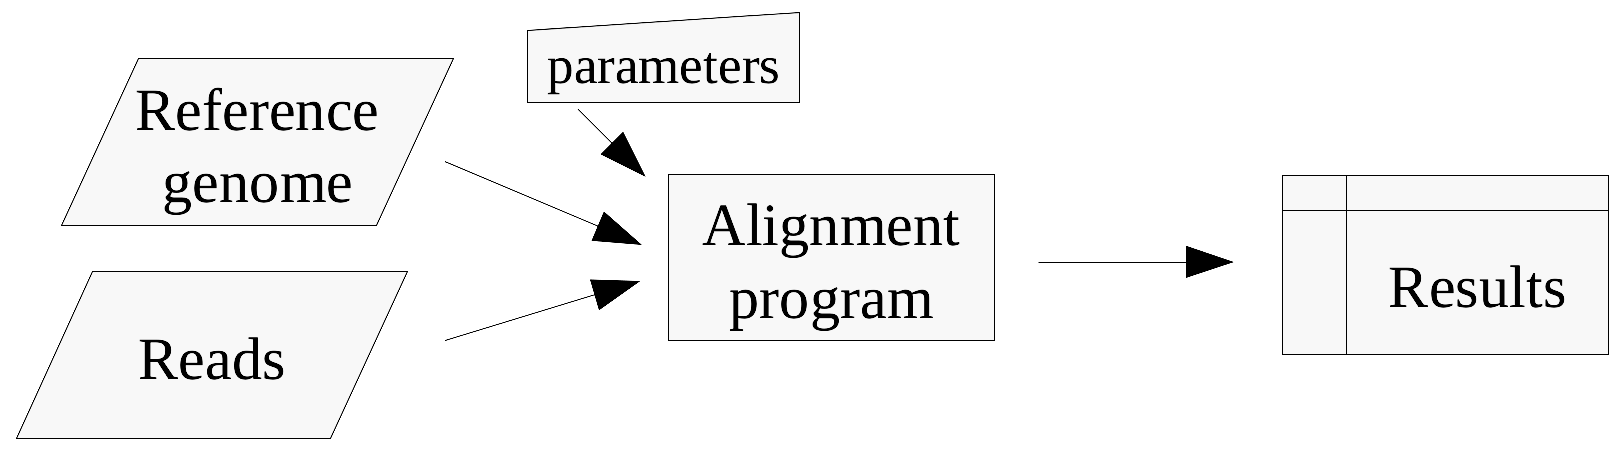
\includegraphics[scale=0.25]{alignreference}
  \caption{alignment of reads on a reference genome}
  \label{fig:alignreference}
\end{figure}

We should consider:
\begin{itemize}
	\item the reference genome
	\item the format and type of the reads to be aligned
	\item the alignment program to use and its parameters 
	\item the format of the result file
\end{itemize}

If the reads must be aligned on a reference genome, then it is important to make sure that the
version of the genome is the one that you want to use.

\subsection{Algorithms to map reads on a reference genome}

da completare

Files used to store aligned data are in SAM and BAM formats.

\paragraph*{Sequence Alignment/Map (SAM) Format}
This specification aims to define a generic nucleotide alignment format, SAM,
that describes the alignment of query sequences or sequencing reads to a
reference sequence or assembly.

\begin{figure}[H]
  \centering
  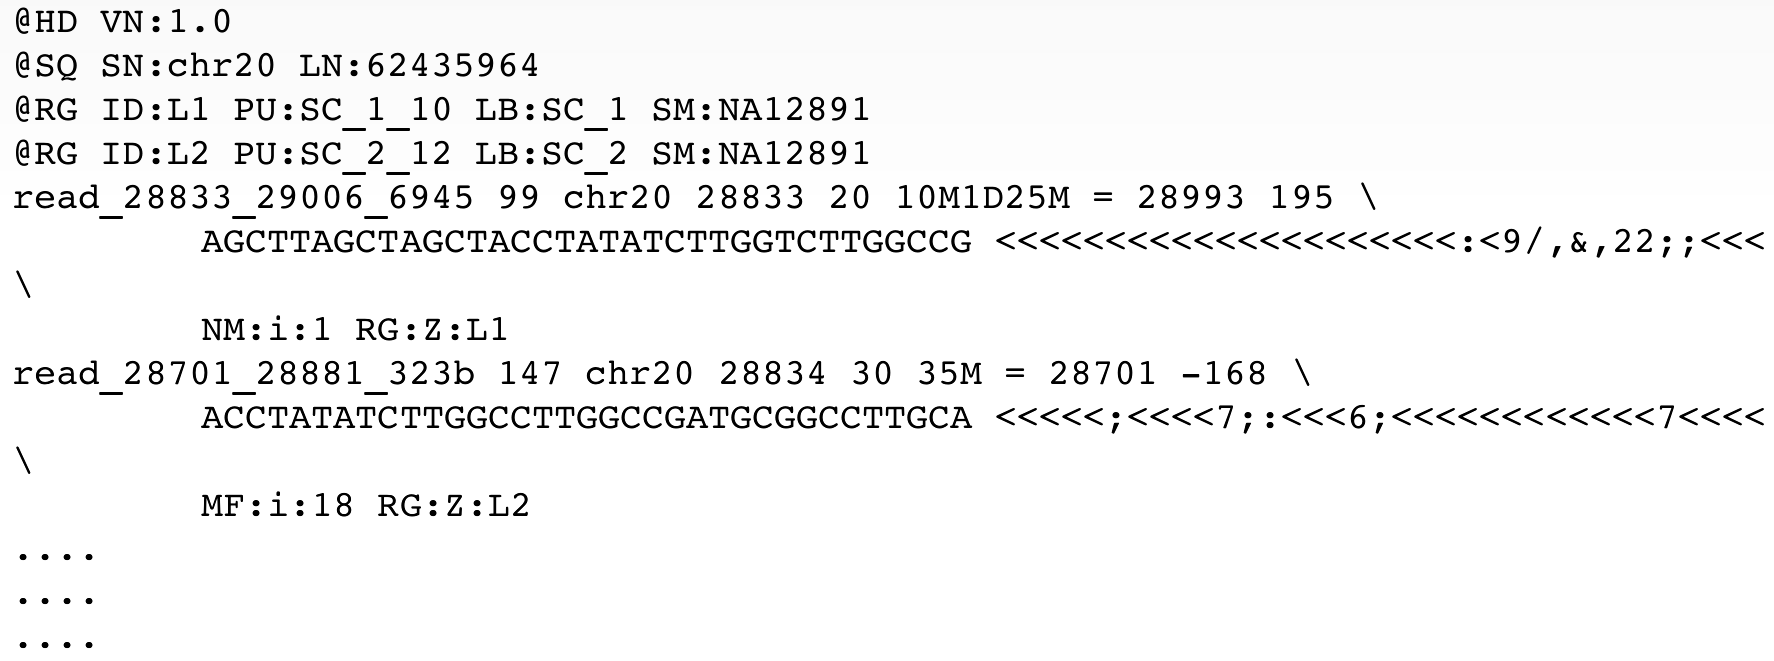
\includegraphics[scale=0.25]{sam}
  \caption{example of sam file}
  \label{fig:sam}
\end{figure}

In a SAM file, all the lines starting with an "@" contain headers information.
After the header section, there is the alignment section consists of multiple TAB-delimited
lines with each line describing an alignment.
